\section{Auswertung}
\label{sec:Auswertung}
\subsection{Bestimmung der Brennweite $f$ über die Messung der Gegenstandsweite $g$ und der Bildweite $b$.}
Zur Bestimmung der Brennweite über die Bildweite und die Gegenstandsweite werden die gemessenen Gegenstandsweiten $g_{\mathrm{i}}$ auf der x-Achse und die gemessenen Bildweiten $b_{\mathrm{i}}$ auf der y-Achse abgetragen und die zueinander gehörigen Datentupel miteinander verbunden.
Die verwendeten Datentupel sind hierbei in Tabelle \ref{tab:bundg} angegeben.
Der sich ergebende Schnittpunkt aller Verbindungsgraden hat schließlich als Koordinaten für beide Raumrichtungen die Brennweite $f$ der verwendeten Linse. Um die Brennweite aus dem Graphen möglichst genau abzulesen, wird der Bereich des Schnittpunkts vergrößert in Abbildung \ref{fig:plota} dargestellt.
Die Brennweite wurde abgelesen zu
\begin{equation}
  f_{\mathrm{abgelesen}}=\SI{9.7(1)}{\centi\meter}\text{.}
\end{equation}
\subsubsection{Experimentelle Überprüfung der Linsengleichung und des Abbildungsgesetz.}
Über die Linsengleichung \eqref{eqn:linsi} ergibt sich über die Mittelung der Brennweiten $f_{\mathrm{i}}$, berechnet aus den Datentupeln aus Bild-und Gegenstandsweite, die Brennweite $f_{\mathrm{Linsengleichung}}$.
Hierbei wird als Fehler, wie in den weiteren Messungen ebenfalls, lediglich der Fehler des Mittelwerts angegeben.
Es ergibt sich
\begin{equation}
  f_{\mathrm{Linsengleichung}}=\SI{9.70(9)}{\centi\meter}\text{.}
\end{equation}

\begin{figure}
  \centering
  \includegraphics{Bilder/plot_a.pdf}
  \caption{Plot.}
  \label{fig:plot}
\end{figure}
Ein Vergleich mit dem aus dem Graphen abgelesenen $f_{\mathrm{abgelesen}}$ zeigt, dass die Linsengleichung für unsere Messung bestätigt werden kann.


\begin{table}
  \caption{Abgelesene Datenpaare aus Bildweite $b$ und Gegenstandsweite $g$.}
  \label{tab:bundg}
  \centering
  \begin{tabular}{ccc}
    \toprule
  b & g & f \\
\midrule
  19.8+/-0.1 & 19.2+/-0.1 & 9.748+/-0.035 \\
  33.7+/-0.1 & 13.3+/-0.1 & 9.54+/-0.05 \\
  21.8+/-0.1 & 17.4+/-0.1 & 9.68+/-0.04 \\
  15.6+/-0.1 & 25.8+/-0.1 & 9.72+/-0.04 \\
  14.0+/-0.1 & 31.0+/-0.1 & 9.64+/-0.05 \\
  100.5+/-0.1 & 11.0+/-0.1 & 9.91+/-0.08 \\
  16.1+/-0.1 & 24.4+/-0.1 & 9.70+/-0.04 \\
  13.8+/-0.1 & 33.3+/-0.1 & 9.76+/-0.05 \\
  13.0+/-0.1 & 37.9+/-0.1 & 9.68+/-0.06 \\
  13.7+/-0.1 & 32.8+/-0.1 & 9.66+/-0.05 \\
\bottomrule
\end{tabular}
\end{table}
Zur Überprüfung des Abbildungsgesetzes werden zudem die Bildgrößen $B$ und Gegenstandsgrößen $G$ benötigt. Die gemessenen Datentupel finden sich in Tabelle \ref{tab:groesse}
\begin{table}
  \caption{Abgelesene Datenpaare aus Bildgröße $B$ und Gegenstandsgröße $G$.}
  \label{tab:groesse}
  \centering
\begin{tabular}{cccccc}
  \toprule
b & g & B & G & V=b/g & V=B/G \\
\midrule
19.8+/-0.1 & 19.2+/-0.1 & 3.0+/-0.1 & 3.0+/-0.1 & 1.031+/-0.007 & 1.00+/-0.05 \\
33.7+/-0.1 & 13.3+/-0.1 & 7.4+/-0.1 & 3.0+/-0.1 & 2.534+/-0.020 & 2.47+/-0.09 \\
21.8+/-0.1 & 17.4+/-0.1 & 3.7+/-0.1 & 3.0+/-0.1 & 1.253+/-0.009 & 1.23+/-0.05 \\
15.6+/-0.1 & 25.8+/-0.1 & 1.9+/-0.1 & 3.0+/-0.1 & 0.605+/-0.005 & 0.63+/-0.04 \\
14.0+/-0.1 & 31.0+/-0.1 & 1.5+/-0.1 & 3.0+/-0.1 & 0.4516+/-0.0035 & 0.50+/-0.04 \\
\bottomrule
\end{tabular}
\end{table}

Vklein= 1.2+/-0.7
Vgroß= 1.2+/-0.7


\subsection{Bestimmung der Brennweite mit der Methode von Bessel}
\begin{table}
  \centering
\begin{tabular}{ccccc}
  \toprule
b1 & g1 & e1 & d1 & f1 \\
\midrule
37.1+/-0.1 & 13.4+/-0.1 & 50.50+/-0.14 & -23.70+/-0.14 & 9.84+/-0.05 \\
46.2+/-0.1 & 12.4+/-0.1 & 58.60+/-0.14 & -33.80+/-0.14 & 9.78+/-0.06 \\
51.6+/-0.1 & 12.0+/-0.1 & 63.60+/-0.14 & -39.60+/-0.14 & 9.74+/-0.07 \\
30.1+/-0.1 & 14.5+/-0.1 & 44.60+/-0.14 & -15.60+/-0.14 & 9.79+/-0.05 \\
41.9+/-0.1 & 12.7+/-0.1 & 54.60+/-0.14 & -29.20+/-0.14 & 9.75+/-0.06 \\
22.0+/-0.1 & 17.6+/-0.1 & 39.60+/-0.14 & -4.40+/-0.14 & 9.78+/-0.04 \\
52.6+/-0.1 & 12.0+/-0.1 & 64.60+/-0.14 & -40.60+/-0.14 & 9.77+/-0.07 \\
39.7+/-0.1 & 12.9+/-0.1 & 52.60+/-0.14 & -26.80+/-0.14 & 9.74+/-0.06 \\
35.0+/-0.1 & 13.6+/-0.1 & 48.60+/-0.14 & -21.40+/-0.14 & 9.79+/-0.05 \\
27.5+/-0.1 & 15.1+/-0.1 & 42.60+/-0.14 & -12.40+/-0.14 & 9.75+/-0.04 \\
\bottomrule
\end{tabular}
\end{table}
\begin{table}
  \centering
\begin{tabular}{ccccc}
  \toprule
b2 & g2 & e2 & d2 & f2 \\
\midrule
13.3+/-0.1 & 37.2+/-0.1 & 50.50+/-0.14 & 23.90+/-0.14 & 9.80+/-0.05 \\
12.0+/-0.1 & 46.6+/-0.1 & 58.60+/-0.14 & 34.60+/-0.14 & 9.54+/-0.06 \\
12.0+/-0.1 & 51.6+/-0.1 & 63.60+/-0.14 & 39.60+/-0.14 & 9.74+/-0.07 \\
14.4+/-0.1 & 30.2+/-0.1 & 44.60+/-0.14 & 15.80+/-0.14 & 9.75+/-0.05 \\
12.7+/-0.1 & 41.9+/-0.1 & 54.60+/-0.14 & 29.20+/-0.14 & 9.75+/-0.06 \\
17.3+/-0.1 & 22.3+/-0.1 & 39.60+/-0.14 & 5.00+/-0.14 & 9.74+/-0.04 \\
11.8+/-0.1 & 52.8+/-0.1 & 64.60+/-0.14 & 41.00+/-0.14 & 9.64+/-0.07 \\
12.9+/-0.1 & 39.7+/-0.1 & 52.60+/-0.14 & 26.80+/-0.14 & 9.74+/-0.06 \\
13.4+/-0.1 & 35.2+/-0.1 & 48.60+/-0.14 & 21.80+/-0.14 & 9.71+/-0.05 \\
15.1+/-0.1 & 27.5+/-0.1 & 42.60+/-0.14 & 12.40+/-0.14 & 9.75+/-0.04 \\
\bottomrule
\end{tabular}
\end{table}
f1= 9.772+/-0.031
f2= 9.71+/-0.07
\subsubsection{Untersuchung der chromatischen Abberation}
\begin{table}
  \centering
\begin{tabular}{ccccc}
  \toprule
b1 & g1 & e1 & d1 & f1 \\
\midrule
37.2+/-0.1 & 13.3+/-0.1 & 50.50+/-0.14 & -23.90+/-0.14 & 9.80+/-0.05 \\
46.3+/-0.1 & 12.3+/-0.1 & 58.60+/-0.14 & -34.00+/-0.14 & 9.72+/-0.06 \\
51.5+/-0.1 & 12.1+/-0.1 & 63.60+/-0.14 & -39.40+/-0.14 & 9.80+/-0.07 \\
30.2+/-0.1 & 14.4+/-0.1 & 44.60+/-0.14 & -15.80+/-0.14 & 9.75+/-0.05 \\
41.8+/-0.1 & 12.8+/-0.1 & 54.60+/-0.14 & -29.00+/-0.14 & 9.80+/-0.06 \\
\bottomrule
\end{tabular}
\end{table}
\begin{table}
  \centering
\begin{tabular}{ccccc}
  \toprule
b2 & g2 & e2 & d2 & f2 \\
\midrule
13.2+/-0.1 & 37.3+/-0.1 & 50.50+/-0.14 & 24.10+/-0.14 & 9.75+/-0.05 \\
12.1+/-0.1 & 46.5+/-0.1 & 58.60+/-0.14 & 34.40+/-0.14 & 9.60+/-0.06 \\
12.1+/-0.1 & 51.5+/-0.1 & 63.60+/-0.14 & 39.40+/-0.14 & 9.80+/-0.07 \\
14.3+/-0.1 & 30.3+/-0.1 & 44.60+/-0.14 & 16.00+/-0.14 & 9.72+/-0.05 \\
12.7+/-0.1 & 41.9+/-0.1 & 54.60+/-0.14 & 29.20+/-0.14 & 9.75+/-0.06 \\
\bottomrule
\end{tabular}
\end{table}

f1 blau= 9.773+/-0.033
f2 blau= 9.72+/-0.07
\begin{table}
  \centering
\begin{tabular}{ccccc}
  \toprule
b1 & g1 & e1 & d1 & f1 \\
\midrule
37.0+/-0.1 & 13.5+/-0.1 & 50.50+/-0.14 & -23.50+/-0.14 & 9.89+/-0.05 \\
46.1+/-0.1 & 12.5+/-0.1 & 58.60+/-0.14 & -33.60+/-0.14 & 9.83+/-0.06 \\
51.5+/-0.1 & 12.1+/-0.1 & 63.60+/-0.14 & -39.40+/-0.14 & 9.80+/-0.07 \\
29.9+/-0.1 & 14.7+/-0.1 & 44.60+/-0.14 & -15.20+/-0.14 & 9.85+/-0.05 \\
41.7+/-0.1 & 12.9+/-0.1 & 54.60+/-0.14 & -28.80+/-0.14 & 9.85+/-0.06 \\
\bottomrule
\end{tabular}
\end{table}
\begin{table}
  \centering
\begin{tabular}{ccccc}
  \toprule
b2 & g2 & e2 & d2 & f2 \\
\midrule
13.4+/-0.1 & 37.1+/-0.1 & 50.50+/-0.14 & 23.70+/-0.14 & 9.84+/-0.05 \\
12.2+/-0.1 & 46.4+/-0.1 & 58.60+/-0.14 & 34.20+/-0.14 & 9.66+/-0.06 \\
11.9+/-0.1 & 51.7+/-0.1 & 63.60+/-0.14 & 39.80+/-0.14 & 9.67+/-0.07 \\
14.5+/-0.1 & 30.1+/-0.1 & 44.60+/-0.14 & 15.60+/-0.14 & 9.79+/-0.05 \\
12.6+/-0.1 & 42.0+/-0.1 & 54.60+/-0.14 & 29.40+/-0.14 & 9.69+/-0.06 \\
\bottomrule
\end{tabular}
\end{table}

f1 rot = 9.846+/-0.030
f2 rot= 9.73+/-0.07
%\begin{figure}
%  \centering
%  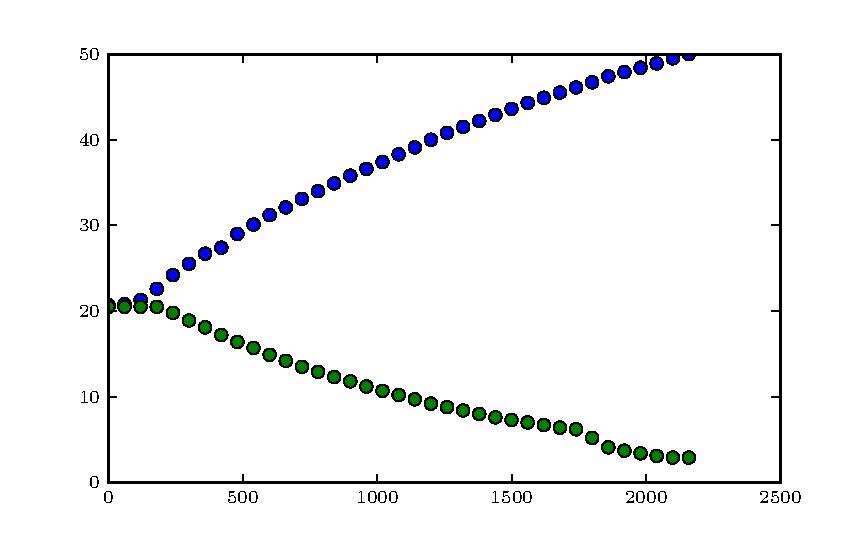
\includegraphics{plot.pdf}
%  \caption{Plot.}
%  \label{fig:plot}
%\end{figure}
